\section{SeismicSpider}\label{sec:SeismicSpider}

Traditional geophones are mounted in an insulated shock resistive enclosure on a spike. The spikes, varying in length, are inserted into the ground to ensure a firm coupling with the environment. The design of our Seismic Spider prevents full depth insertion of the three inch spikes. 

	To overcome the coupling issue we are using three geophones per station compared to the typical one. Our immediate goals are to compare amplitude and phase response to that of a standard single station.	

\begin{figure} \centering
  {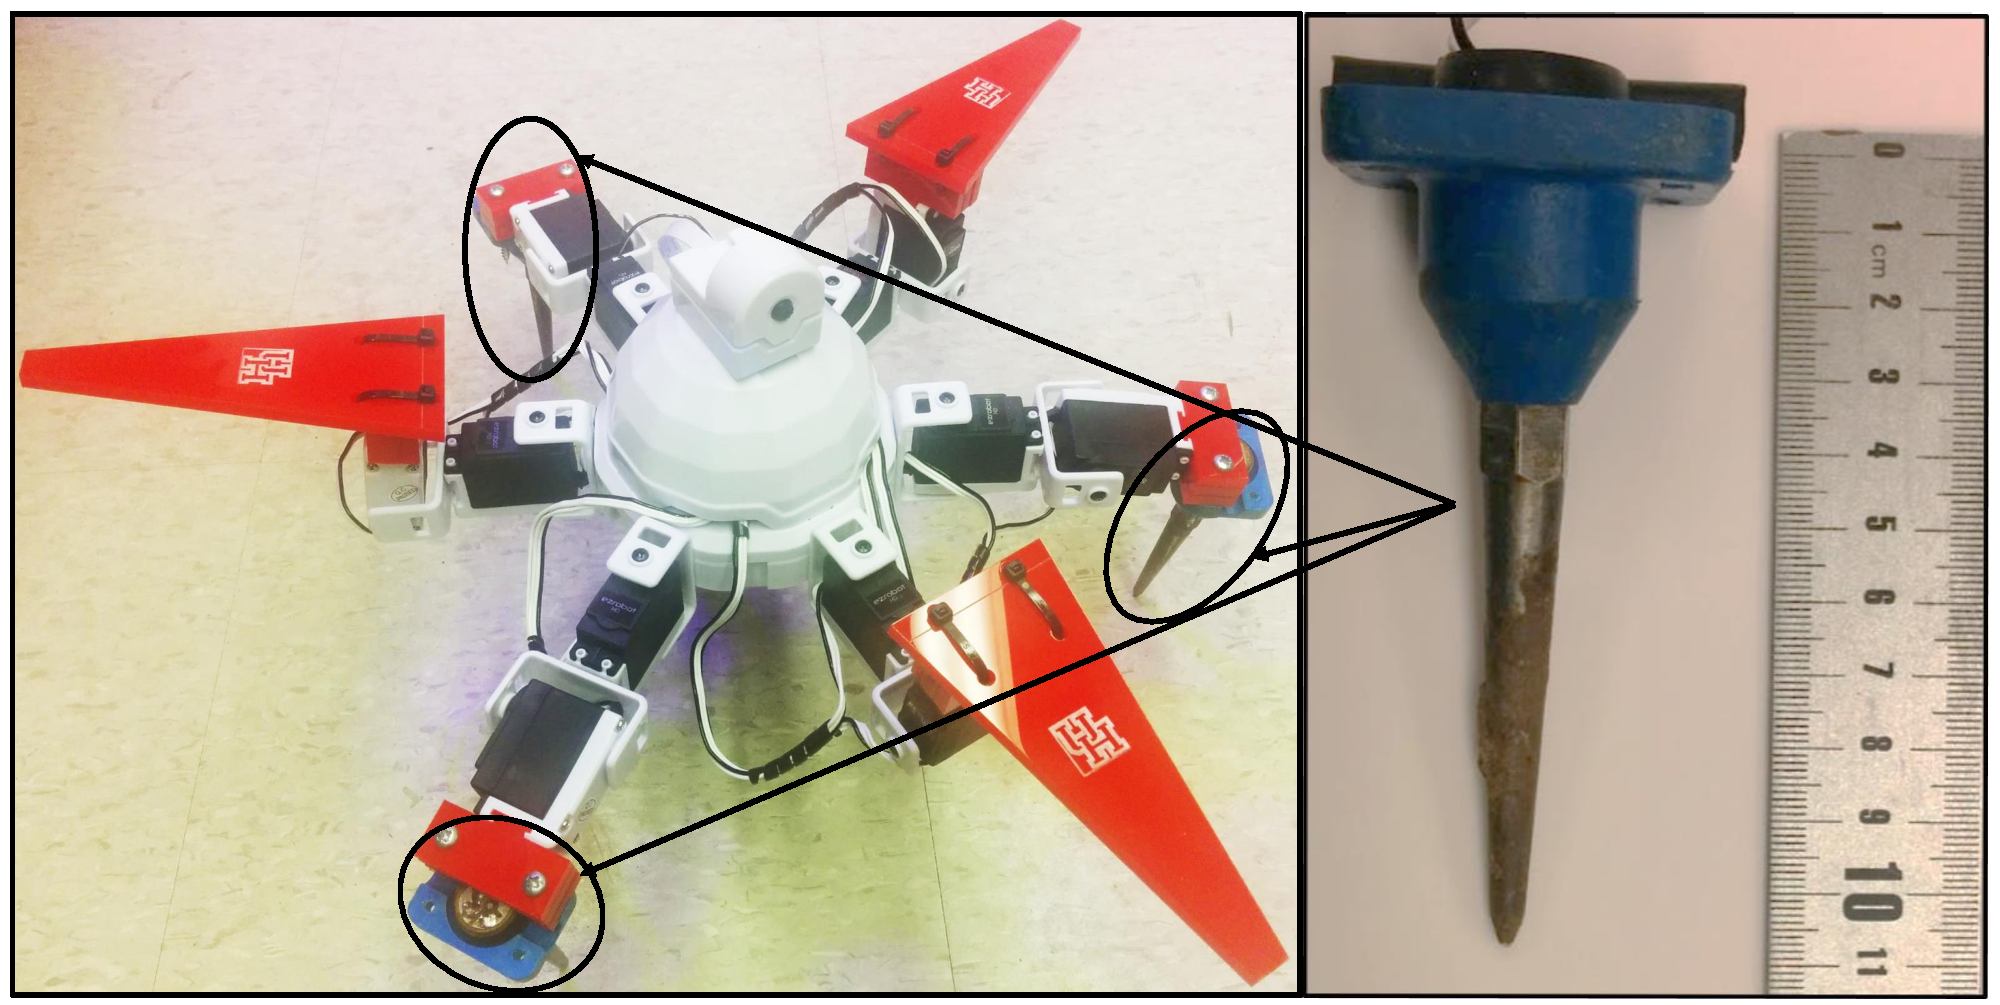
\includegraphics[width=\columnwidth]{Hex_overview.pdf}}
 \caption{The SeismicSpider is a six-legged mobile robot where three legs are replaced by geophones. It senses and records seismic data.} 
 \label{fig:TradvsAutoDrop}
\end{figure}
\subsection{Design}

The Seismic Spider is built from the Six Hexapod kit designed by EZ Robots. Each of the six legs are powered by two 15 kg/cm lever servos. The peg legs were replace by three GS-20DM 14 Hz geophones from Geospace Technologies. The remaining three were designed to match the geophone dimensions and reflect UH school spirit.

 Our initial plan to use three geophones require the spider to raise the three inactive legs while acquiring data. This lack of support caused excessive strain on the three servo motors responsible for holding the spider upright introducing unwanted vibration into the system. We found positioning the geophone legs at 20$^\circ$ to normal enhanced the stability and relieved the excessive stress on the servos. 
 The three geophones were in series, so with each geophone leg angled inward, superposition replicates the signal from one vertical geophone.

\subsection{Shot gather comparison}
%\subsubsection{Accuracy plot}
%Hexapod move to desired GPS location  (plot accuracy)\\
%\subsubsection{ Shot gather comparison}

A line of twenty four geophones, GS-20DM 14 Hz, were laid out at one meter intervals with our inline source seven meters from the nearest geophone. Beginning from the farthest offset of 31 meters we manually aligned the Spider with the corresponding geophone, fired the source, then moved one meter ahead. 

%\paragraph{Results}
Data from the shot gather comparison is shown in Fig.~\ref{fig:shotgatherHexpod}.
We found a correlation, unmeasured, with the standard geophones and we more than compensated for loss of amplitude with three geophones, the response was 5 dB greater that the single geophone. The geophone wires proved insufficient to insulate against 60 Hz. Hence the raw data from the traditional setup as well as the Seismic Spider was trough a (3-50) band-pass filter. Further the SeismicSpider data was attenuated by $-5$dB to level the comparison.  Due to the small amount of usable data we were not able to gain meaningful results for phase analysis.   

\begin{figure} \centering
  {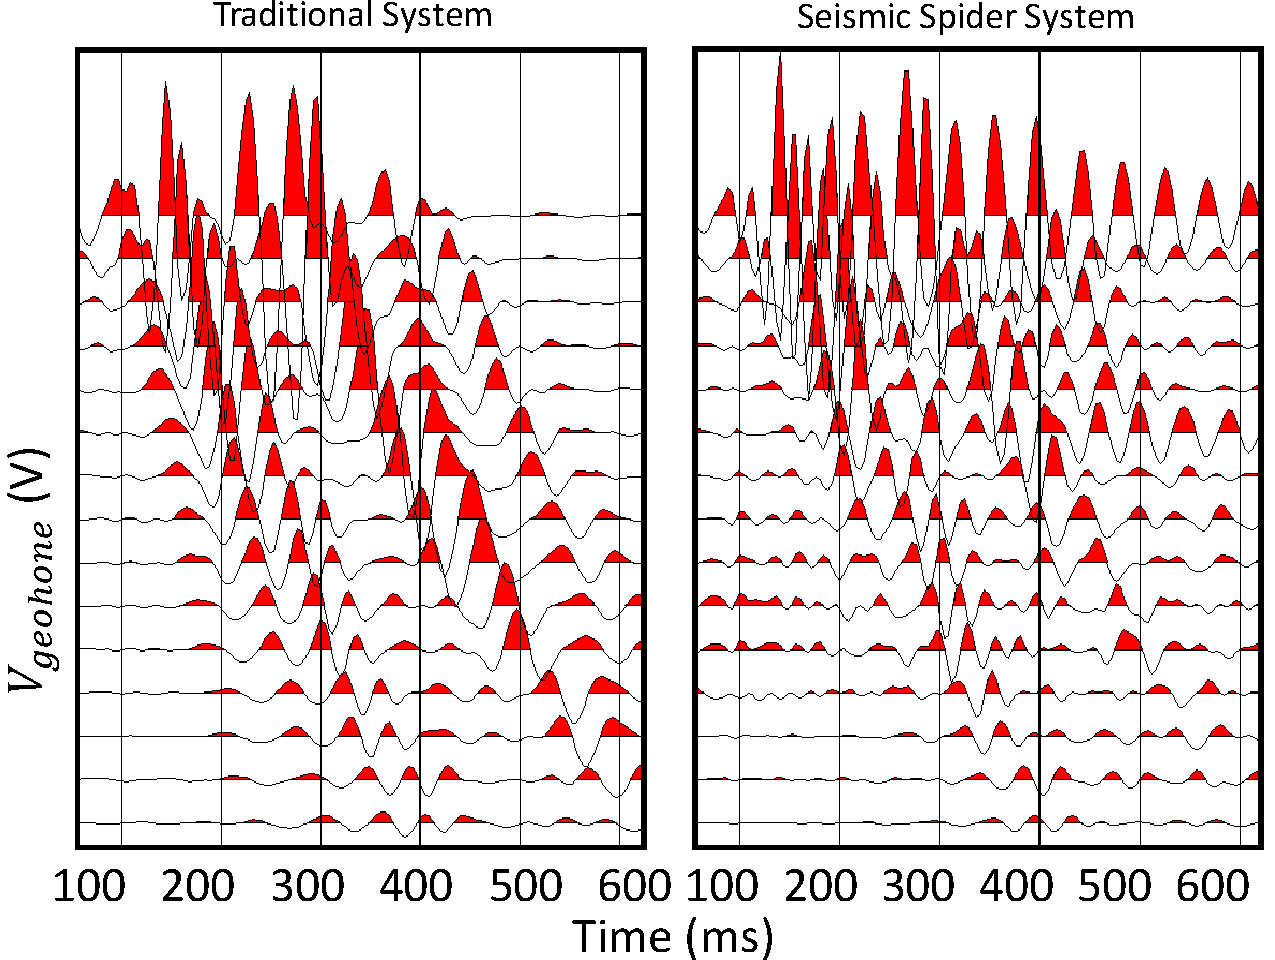
\includegraphics[width=\columnwidth]{shotgather_hex.pdf}}
 \caption{Shot gather comparison of traditional geophones vs. hexapod sensor. 
 \label{fig:shotgatherHexpod}}
\end{figure}

%\paragraph{Future work}	we must filter 60 Hz noise, compare adding geophones to all six legs, and design a larger seismic survey to ensure adequate data for phase analysis. Design improvements could be done to make the SeismicSpider an active sensor.   

\subsection{Deploying and Retrieving Hexapod}
\begin{figure} \centering
  {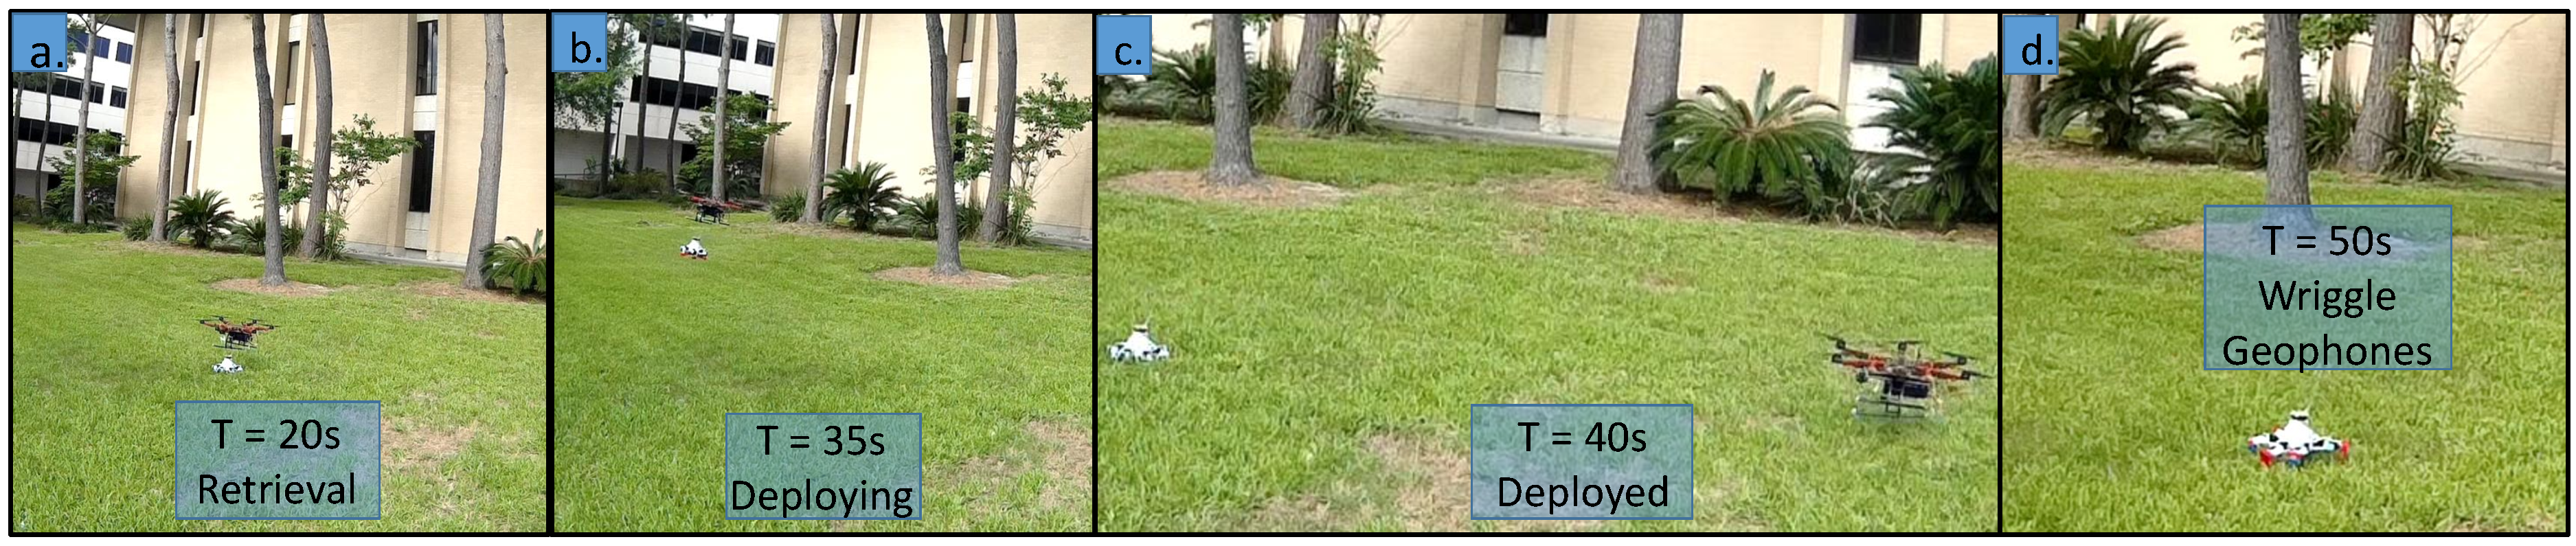
\includegraphics[width=\columnwidth]{SeismicSpider_DR.pdf}}
 \caption{Shot gather comparison of traditional geophones vs. hexapod sensor. 
 \label{fig:SeismicSpider_DR}}
\end{figure}
The Seismic UAV’s purpose is to deploy sensors at respective GPS waypoint locations. The SeismicSpider is a mobile robot, but it’s substantially slower compared to the UAV. Fig.~\ref{fig:SeismicSpider_DR} shows the SeismicSpider being deployed and retrieved from a location. The UAV carrying the SeismicSpider was manually piloted to a specific location. The deployment mechanism included a hook controlled by a servo attached to the UAV. The altitude was carefully lowered and the SeismicSpider was placed on to the ground, then the servo was triggered to unhook the sensor.  The SeismicSpider was sprung to life using a mobile application. The SeismicSpider was controlled to wriggle its three standard legs to plant it’s  geophone legs into the ground.  The SeismicSpider has an onboard GPS that could be used to navigate to a specific waypoint.  Currently autonomous deployment of sensors is possible whereas the retrieval is piloted. Combing the mobility of the Seismic Spider with the speed of the UAV, locations that are inaccessible by air or impossible to penetrate by SmartDarts could be tackled with ease.
